% Chapter 01

\chapter{Introduction}\label{ch:intro}
As the most abundant protein in most eukaryotic cells, actin participates in more protein-protein interactions than any known protein \citep{dominguez_actin_2011}. All eukaryotes have have at least one gene for actin and many have complex actin networks with only a single actin gene, such as budding yeast, fission yeast, and green algae \citep{pollard_actin_2016}. However, some species have many actin genes that are expressed in different tissues. For example, Humans have three genes for $\alpha$-actin, one gene for $\beta$-actin, and two genes for $\gamma$-actin and plants can have 10 or more actin genes \citep{pollard_actin_2016}. Additionally actin is highly conserved among organisms and, even among the three isoforms ($\alpha, \beta, \gamma$-actin) in vertebrates, only varies by a few amino acids near the N-terminus \citep{dominguez_actin_2011}. The actin cytoskeleton plays many biochemical and mechanical roles in the cell and is important for many cellular processes such as polarity establishment, motility, and morphogenesis \citep{blanchoin_actin_2014}. To fulfill these roles, the actin cytoskeleton forms distinct and dynamic networks made up of filamentous actin (F-actin) and other actin binding proteins (ABPs). These networks are formed and degraded at certain times and locations within cells for proper cellular function. 

\section{Actin}\label{actin-intro}

Actin is a 46 kDa globular protein and contains four subdomains. The N-terminus is located in subdomain 1, then the polypeptide domain proceeds through subdomains 2, 3, and 4, returning to subdomain 1 with the C-terminus \citep{pollard_actin_2016}. Subdomains 1 and 3 are structurally similar though contain little sequence similarity \citep{dominguez_actin_2009,pollard_actin_2016}. Subdomains 1 and 2 form the outer domain while 3 and 4 form the inner, larger domain. Between these domains is a hinge region and two large clefts, a nucleotide binding cleft and a target binding cleft. The nucleotide binding cleft binds ATP and an associated cation (Mg\textsubscript{2+} in cells). Many proteins bind actin in the target binding cleft between subdomains 1 and 3 \citep{dominguez_actin_2009}.

Actin assembles into polar filaments with new subunits being primarily added onto the barbed end (subdomains 1 and 3) versus the pointed end (subdomains 2 and 4). The polarity of the filaments was initially observed when visualizing actin filaments saturated with myosin heads using electron microscopy \citep{huxley_electron_1963}. The myosin heads formed an arrowhead-shaped object and thus defined the "barbed" and "pointed" end of the filament due to which direction the arrowheads were pointing. An actin filament contains two protofilaments that wrap around each other with a right-handed twist along the long-axis \citep{hanson_structure_1963}. However, the repeated unit of symmetry is a left-handed helix with \mytilde13 actin subunits repeating every 35.9 nm. The G-actin to F-actin transition consists of a 12-13$^\circ$ rotation of the outer domain (subunits 1 and 2) with respect to the inner domain (subunits 3 and 4) with some additional bending movements of subdomains 2 and 4. Therefore, F-actin is flatter than F-actin and the D-loop in subdomain 2 inserts into the target-binding cleft of the subunit above \citep{dominguez_actin_2011}.

Actin monomers bind both ATP or ADP tightly and a nucleotide-free G-actin will rapidly acquire ATP with a Kd in the nanomolar range \citep{de_la_cruz_nucleotide-free_1995}. A bound nucleotide stabilizes an actin monomer, but is not required for polymerization \citep{pollard_actin_2016}. Monomers polymerize spontaneously under physiological salt conditions with cations present. This spontaneous assembly has an initial lag period due to the slow nucleation step caused by the instability of actin dimers and trimers \citep{cooper_kinetic_1983, frieden_polymerization_1983, sept_thermodynamics_2001}. Once the fourth subunit has been added to the actin nucleus, the seed is more stable and elongation occurs at the same rate as longer filaments. Barbed ends elongate 10 times faster than pointed ends. ATP-actin associates with barbed ends with a rate constant of \mytilde10 $\mu$M\textsubscript{-1} s\textsuperscript{-1} and slowly dissociates at \mytilde 1 s\textsuperscript{-1} \citep{pollard_rate_1986}. Thus the 'critical concentration' for monomer addition is 0.1 $\mu$M for the barbed end of actin filaments. Once a monomer undergoes the conformational change to bind to a filament, the rate of hydrolysis increases to 0.3 s\textsuperscript{-1}. Hydrolysis is thought to occur randomly along the filament \citep{jeno_internal_1995}, though it has been proposed that neighboring subunits could effect the rate \citep{korn_actin_1987}. Once hydrolysis occurs, the phosphate is slow to dissociate \citep{carlier_direct_1986}, leaving ADP-actin which dissociates more easily from both ends. 

The total cellular concentration of actin is between 50-200 $\mu$M. In cells, filaments assemble and disassemble on the timescale of tens of seconds. Actin binding proteins (ABPs) cause large differences from the \textit{in vitro} rates and allow for almost half of the total actin in cells to be unpolymerized (\mytilde25-100 $\mu$M) which is far above the critical concentration. Within cells there is millimolar concentrations of Mg-ATP and phosphate, so most cytoplasmic G-actin has bound Mg-ATP. Once the G-actin is added to F-actin, the Mg-ATP is hydrolyzed and then the phosphate is released. Depolymerization of F-actin releases Mg-ADP monomers, where ADP is exchanged for ATP. The ADP to ATP exchange is slow, but can be sped up by an actin monomer binding protein, profilin \citep{pollard_actin_2016}. The rates are further changed by ABPs that nucleate, elongate, cap, sever, and crosslink filaments. 

\begin{figure}
\centering
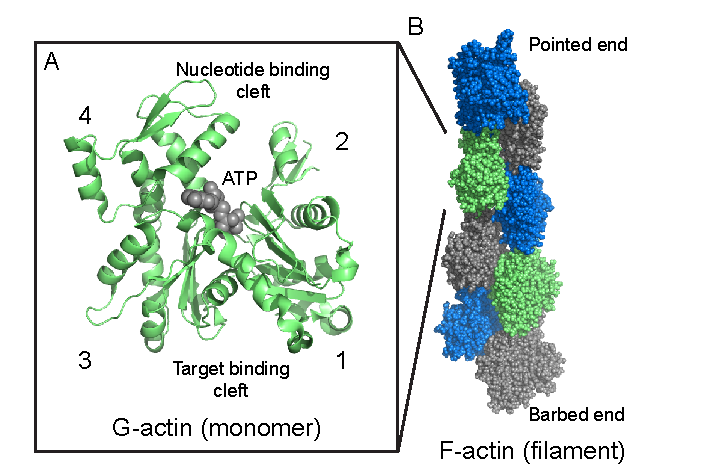
\includegraphics[width=17cm]{img/ch01/actin_thesis.pdf}
\caption[Monomeric G-actin is assembled into filamentous F-actin.]{\textbf{Monomeric G-actin is assembled into filamentous F-actin.} (A) Monomeric globular actin (G-actin) (PDB: 1NWK) contains four subdomains with the N- and C-terminus in subdomain 1. In the center  binding clefts for a nucleotide and other actin binding proteins in the target binding cleft. G-actin assembles into filamentous actin (F-actin) (PDB: 6BNO) that is polar with a fast growing barbed end and a slow growing pointed end.}
\label{fig:actin-structure}
\end{figure}

\section{Actin networks}\label{network-intro}
The actin filaments in cells are organized into distinct, dynamic networks that allow the cell to carry out processes such as cytokinesis, endocytosis, motility, and adherence. A set of ABPs localize to each distinct network, which allows for each network's unique architecture and function. One simplified model organism, S. Pombe fission yeast, only has one actin isoform, yet has three distinct actin networks: actin patches for endocytosis, actin rings for cytokinesis, and actin cables for polarity establishment. Here I will focus on three actin networks found in higher eukaryotes; lamellipodia, filopodia, and stress fibers. 

\subsection{Lamellipodia}\label{lamellipodia-intro}
The lamellipodium is made of short, branched actin filaments that form a thin, dense meshwork \citep{small_lamellipodium:_2002}. Lamellipodia can extend up to tens of microns along the leading edge of motile cells \citep{skau_specification_2015}. The branched network is nucleated by the Arp2/3 complex, which must be activated by a nucleation promoting factor (NPF) such as WAVE or WASP proteins \citep{blanchoin_actin_2014}. The branches are kept short by capping protein, which blocks barbed end filament growth and filaments are severed for recycling by cofilin. The branched filaments are crosslinked into a dense mesh by the bundling proteins fimbrin, $\alpha$-actinin, and filamin \citep{small_lamellipodium:_2002}. The growth of the dense network pushes on the leading edge membrane generating force. Lamellipodia polymerization drives the membrane forward when membrane tension is low, but drives cell movement when membrane tension is high and the cell is adhered to a surface through retrograde flow \citep{skau_specification_2015}.  

\subsection{Filopodia}\label{filopodia-intro}
The dynamic fingerlike projections that emerge from the lamellipodium are called filopodia. Filopodia are important for exploration of the mechanical and chemical extracellular space of motile cells \citep{mattila_filopodia:_2008}. This is especially important in steering neuronal growth cones, wound healing, and dorsal or ventral closure during development. During these processes cells must be able to follow mechanical and chemical signals in order to move through space towards other cells or locations \citep{bornschlogl_how_2013}. Filopodia are made up of 10-30 tightly packed filaments, primarily bundled by crosslinking protein, fascin \citep{vignjevic_role_2006, mellor_role_2010}. These filaments form parallel bundles, with all their barbed ends organized towards the tip of the filopodia \citep{bornschlogl_how_2013}.

There are two proposed models for how filopodia form at the leading edge of cells: convergent elongation \citep{yang_filopodia_2011} and de-novo nucleation \citep{faix_filopodia:_2009} (Figure \ref{fig:filopodia-init}). The convergent elongation model proposes that the filaments for filopodia are initially nucleated by Arp2/3 complex in the lamellipodia. These filaments make $\lambda$-shaped precursors that can then be bundled by fascin \citep{svitkina_mechanism_2003,small_lamellipodium:_2002}. In contrast, the de-novo nucleation proposes that filopodia formation is distinct from the lamellipodium and nucleation of these filaments is facilitated by formins such as mDia2 \citep{faix_making_2006,mellor_role_2010}. It could be that different nucleators are driving different types of filopodia in different cell types. Futhermore, some cells can produce different types of filopodia within the same cell. For example, S2 cells from \textit{Drosophila} have short, more dynamic filopodia formed by Ena compared to formin Dia \citep{bilancia_enabled_2014}. This is also seen in mammalian cells where VASP or mDia2 expression facilitates varying number of filopodia with different dynamics and morphology \citep{barzik_ena/vasp_2014}. 

\begin{figure}
\centering
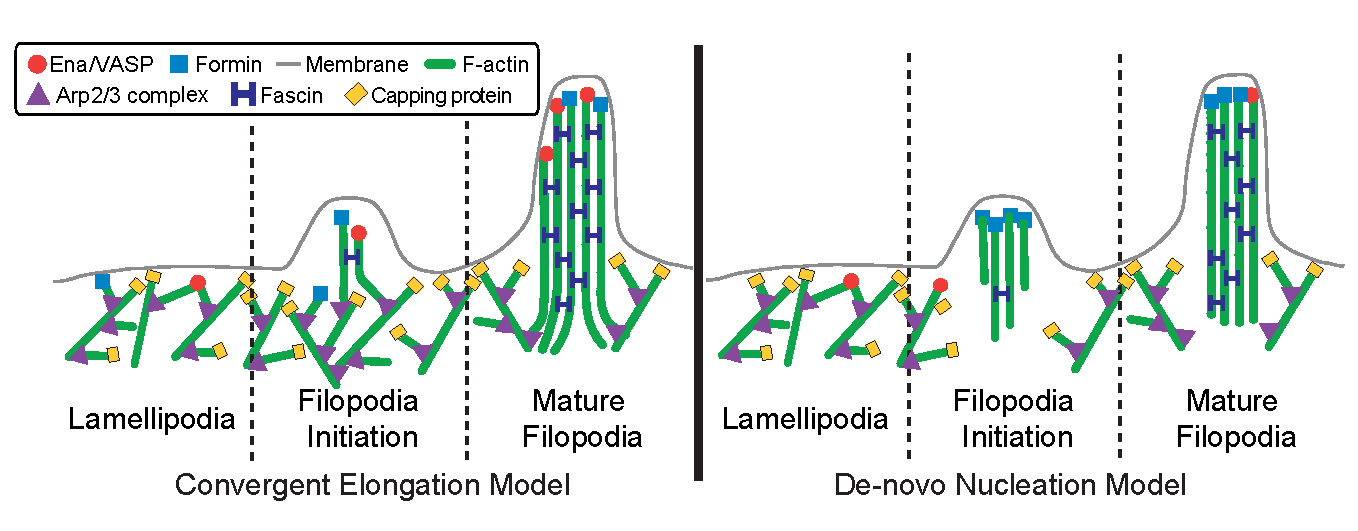
\includegraphics[width=\textwidth]{img/ch01/filopodia_comparison_thesis.pdf}
\caption[Comparison of models for filopodia formation.]{\textbf{Comparison of models for filopodia formation.} A comparison between two models for filopodia formation. The convergent elongation model (left) proposes that filaments are nucleated by Arp2/3 within the lamellipodia and are gathered into parallel fascin-mediated bundles by elongation factors Ena/VASP and formin. The de-novo nucleation model (right) postulates that nucleation of filopodia filaments occur at the membrane by nucleation factors such as formin and are separate from the Arp2/3 nucleated filaments in the lamellipodia.}
\label{fig:filopodia-init}
\end{figure}

\subsection{Stress Fibers}\label{stressfibers-intro}
Another way that cells can produce force through actin networks is contractile stress fibers. Stress fibers are formed from actinmyosin bundles formed mainly by $\alpha$-actinin. There are three main types of stress fibers in animal cells: ventral, dorsal, and transverse arcs. Ventral stress fibers are anchored at each end by focal adhesions where dorsal stress fibers are only anchored at one end near the leading edge. Transverse arcs are convex stress fibers that form parallel to the leading edge \citep{burridge_focal_2016}. Stess fibers and focal adhesions are important for cell adhesion, morphogenesis, and especially mechanotransduction \citep{tojkander_actin_2012}. Stress fibers are the main vehicle for contractile forces in cells. The contractile force is formed by myosin II that binds alternating with $\alpha$-actinin along the stress fibers \citep{naumanen_mechanisms_2008}. 

\section{Actin binding proteins}\label{abps} 
Actin binding proteins (ABPs) can nucleate, elongate, cap, sever, disassemble, and crosslink F-actin. ABPs also can bind to actin monomers, such as profilin. Profilin is a small actin binding protein that has high affinity for ATP-actin monomers (Kd = 0.1 $\mu$M) \citep{pollard_actin_2016}. However, profilin binds monomers on the barbed end so it inhibits nucleation and elongation at the pointed end, though allows elongation at barbed ends. When a profilin-actin complex binds the barbed end, the conformational change in the actin subunit decreases profilin's affinity facilitating dissociation. Profilin is also important for catalyzing nucleotide exchange in actin monomers \citep{mockrin_acanthamoeba_1980, vinson_interactions_1998}. Between profilin and another actin monomer binding protein, thymosin-$\beta$4, there is a low concentration of free actin monomers \citep{pollard_actin_2016}.

Other ABPs can bind to sides of F-actin, such as tropomyosin and myosin. Tropomyosin is a coiled-coil protein that binds along the long-pitch helices of F-actin \citep{ecken_structure_2015}. Tropomyosin stabilizes filaments and increases its persistence length \citep{sousa_electron_2010}. Additionally, in muscle cells tropomyosin regulates the binding of myosin. Myosin is a family of ATP-motors that bind and release actin filaments throughout the ATP hydrolysis cycle. Depending on the type of myosin, this allows processive runs along actin filaments or muscle contraction in sarcomeres. Myosins are important for force generation, transport of cargo along F-actin, anchoring organelles, and mechanotransduction \citep{hartman_myosin_2012}.

\subsection{Nucleation factors}\label{nucleators}
As described earlier, actin nucleation is slow; therefore, in cells ABPs catalyze the formation of an F-actin seed. There are three different classes of these nucleation factors. The first class is the Arp2/3 complex. The Arp2/3 complex is made up of seven subunits including Arp2 and Arp3, which are actin related proteins (Arp). Arp2/3 complex nucleates filaments by binding to the side of a mother filament and using its Arp2 and Arp3 proteins to template the nucleation of a filament that branches from the mother at a 70$^{\circ}$ angle. In order to nucleate branches, Arp2/3 needs to be activated via a nucleation promoting factor such as WAVE or WASP. Arp2/3 complex nucleates filaments for the lamellipodia, some stress fibers and actin patches in S. pombe \citep{pollard_actin_2016, naumanen_mechanisms_2008, mishra_yeast_2014}. Recently, it was shown that profilin is antagonistic to Arp2/3 \citep{suarez_profilin_2015,rotty_profilin-1_2015}. Therefore, profilin could play a role in regulating the development of formin networks instead of Arp2/3 complex networks. 

The second class of nucleation factors are formins, which nucleate unbranched filaments. There are still some open questions surrounding how formins nucleate filaments \textit{in vivo}. Initially, it was thought that formins could stabilize actin dimers with their FH2 domain to aid in nucleation, since the FH2 domain is necessary and sufficient for nucleation \textit{in vitro} \citep{zigmond_formin-induced_2004,paul_role_2008,pring_mechanism_2002}. However, it was found that FH2 domains are inefficient at nucleating profilin-actin, which is thought to be the main substrate available \textit{in vivo}. Recently it has been shown that C-terminal tail regions of certain formins, FH1 domains, and NPF that bind to the C-terminal tail region could assist the FH2 domain for profilin-actin nucleation \citep{breitsprecher_formins_2013}. Formins can nucleate filaments for the lamellipodia, filopodia, some stress fibers, and contractile rings \citep{faix_filopodia:_2009,mishra_yeast_2014,blanchoin_actin_2014}.

The third class of nucleation factors are WH2 nucleators. This is a much broader class than the other two classes and contains proteins such as Spire, Cobl, and bacterial VopL and VopF (VopL/F) \citep{quinlan_drosophila_2005, namgoong_mechanism_2011, burke_bacterial_2017,siton-mendelson_functional_2017}. This is a more recently discovered class of nucleators that use tandem WH2 domains to bind and bring together actin monomers to form a nucleus. The proteins in this class have variable nucleation activities, caused by the differences in the number of WH2 domains and also the length of linkers between them \citep{siton-mendelson_functional_2017}. As an example, VopL/F are virulence factors from bacteria \textit{Vibrio parahaemolyticus} and \textit{Vibrio cholera} that can assemble unproductive F-actin in host cells \citep{liverman_arp2/3-independent_2007}. VopL/F contains three tandem WH2 domains and dimerizes through a VopL/F C-terminal domain (VCD). However, two different mechanisms were proposed for VopL and VopF, two closely related proteins. One mechanism suggested that VopL nucleates actin filaments from the pointed end \citep{namgoong_mechanism_2011,yu_mechanism_2011,zahm_bacterial_2013}, while the other mechanism proposed that VopF nucleated filaments then continued to assemble actin at the barbed end, similar to a formin \citep{pernier_dimeric_2013}.

\subsection{Elongation factors}\label{elongators}
Beyond nucleation, there are also assembly factors that aid in actin elongation. Actin will assemble spontaneously at a rate of \mytilde10 $\mu$M s\textsuperscript{-1} \citep{pollard_rate_1986}; however, there are ABPs that associate with the growing barbed end and can change this polymerization rate. Formins are able to increase the elongation rate of F-actin using profilin-actin \citep{pollard_actin_2016}. Another elongation factor protein is Enabled/Vasodilator stimulating phosphoprotein (Ena/VASP). These tetrameric proteins use WH2-like domains to associate with the barbed end and can increase F-actin elongation with both actin and profilin-actin. I will return to these two proteins to look closer into their mechanisms and functions.

\subsection{Bundling proteins}\label{bundlers}
There are different families of proteins that are able to crosslink F-actin. These proteins contain more than one actin binding domain so that they can bind to more than one filament at a time. Crosslinking defined as holding two filaments together at one point. In contrast, bundling is when two filaments are held parallel to each other by multiple crosslinks \citep{pollard_actin_2016}. I will use bundling protein to describe proteins that are able to bundle filaments \textit{in vitro}, though their main function in cells may be to crosslink rather bundle filaments. 

\begin{figure}
\centering
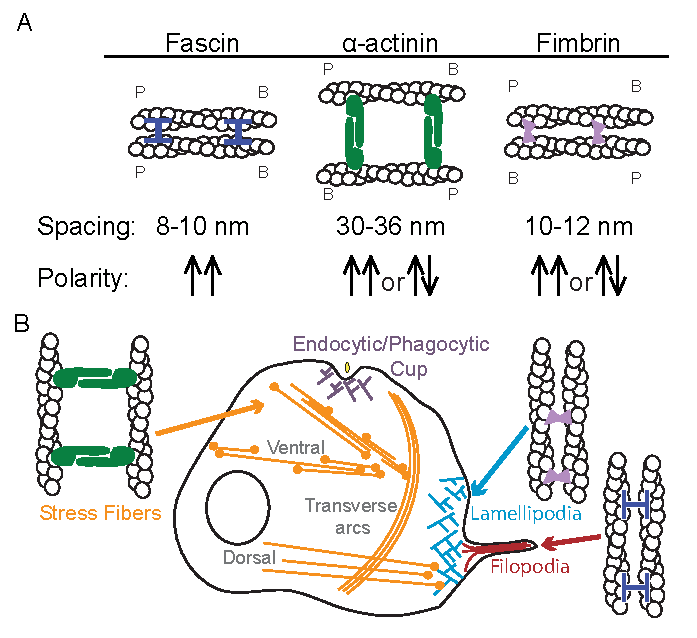
\includegraphics[width=14cm]{img/ch01/bundlers_thesis.pdf}
\caption[Bundling proteins form diverse bundles.]{\textbf{Bundling proteins form diverse bundles.} (A) Fascin forms narrow parallel bundles. $\alpha$-actinin forms wide parallel and antiparallel bundles. Fimbrin forms narrow parallel and antiparallel bundles.(B) Different bundling proteins localize to distinct actin networks. $\alpha$-actinin localizes to stress fibers which include ventral, dorsal, and transverse arcs. Fimbrin localizes predominately to the lamellipodia while fascin is found in filopodia.}
\label{fig:intro-bundlers}
\end{figure}

The largest group of bundling proteins fall in the CH domain superfamily, such as fimbrin/plastin, $\alpha$-actinin, spectrin, and filamin. These proteins use two sets of tandem CH domains to bind to two actin filaments. Fimbrin contains two tandem CH domains to bundle F-actin as a monomer and localizes to the lamellipodia and base of filopodia in cells. Fimbrin bundles have narrow spacing, \mytilde10-12 nm, and can consist of antiparallel and parallel filaments \citep{hanein_atomic_1998}. $\alpha$-actinin also uses CH-domains to bundle actin but only contains one tandem CH domain per monomer so to bundle F-actin it must form a dimer using its spectrin repeats. $\alpha$-actinin bundles have much wider spaced filaments and can also contain either parallel or antiparallel filaments \citep{sjoblom_alpha-actinin_2008}. Different $\alpha$-actinins have slightly different spacing due to the number of spectrin repeats that separate the CH domains. For example, \textit{S. Pombe} Ain1 contains just two spectrin repeats compared to human $\alpha$-actinin IV, which contains four \citep{murphy_actinin_2015}. $\alpha$-actinin and fimbrin bind on the same site of the actin filament \citep{klein_structure_2004}. In contrast, fascin bundles F-actin using its four $\beta$-trefoil domains \citep{jansen_mechanism_2011}. Fascin is a small globular bundling protein that is the main bundling protein in filopodia \citep{vignjevic_role_2006,mellor_role_2010}. Fascin forms bundles that are narrowly spaced, between 8-10 nm, and only consist of parallel filaments \citep{edwards_fascins_1995,jansen_mechanism_2011,cant_drosophila_1994}. 

\section[Ena/VASP and Formins]{Ena/VASP and Formins\footnotemark}\label{ena-formin-review}

\footnotetext{Portions of this section were modified from a review in preparation with Jonathan Winkelman.} 

\subsection{Comparison of processive actin elongation factors}\label{comparison-why}

Mechanistic understanding of the actin cytoskeleton and ABPs is important for understanding how each protein works individually, but also how the different proteins effect each other and contribute to proper function of cellular processes. I am interested in looking at the molecular mechanism of ABPs to understand how proteins are properly functioning, but also how with different diseases and mutations the proteins fail to function. This detailed mechanistic understanding is the foundation that cell biology can be built upon, leading to deeper knowledge of processes that occur in cells and even organisms. 

Here I will focus on the mechanism of two processive protein families, formins and Ena/VASP, which bind to the barbed end of actin filaments and affect actin filament polymerization. Interestingly, though these two families have different structures and use distinct mechanisms, they share similarities in how they increase actin polymerization as well as that they are both localized to the leading edge and involved in filopodia formation. However, their mechanistic differences in terms of processive run lengths, diverse protein binding partners, and formin's reliance on profilin actin bring up many interesting questions concerning how these proteins are utilized by a cell within different and even the same processes. The knowledge of formin's mechanism is a step ahead of Ena/VASP's, exploring the role of force, rotation, and diverse actin regulatory domains on its actin assembly properties. However, this allows insight to compare and contrast the two processive machines and understand how they both individually and concurrently help to assemble the necessary actin networks for proper cellular function. 

\subsection{Cellular processes}\label{ena-formin-cellular-processes}\label{comparison-cellular}

\subsubsection{Formin}

Formin homology proteins (formins) are highly conserved actin binding proteins that function in multiple cellular processes such as cytokinesis, oogenesis, and stress fiber and filopodia formation. Furthermore, formins can interact with both actin and microtubules \citep{bartolini_formin_2008,henty-ridilla_accelerated_2016}, allowing for communication between these two cytoskeleton systems. Formins were first discovered as mutations at the mouse limb deformity (ld) locus resulting in development defects \citep{woychik_formins:_1990}. Since their discovery the formin family has grown, now counting 15 different formins in mammalian cells. The formins are localized to different areas of the cell including the leading edge, tips of filopodia, cell-cell junctions, and cytokinetic rings \citep{pollard_actin_2016}. Formins are implicated in nucleation of nascent actin filaments, processive elongation, and competition with capping protein as well as other F-actin barbed end binding proteins. However, there are some proteins within the formin family (i.e. INF2, Daam1) that have been shown to exhibit additional behaviors, such as depolymerization, bundling of filaments, severing, or actin monomer binding \citep{gurel_assembly_2015}. Though the mechanism of formin's processive F-actin assembly has been well-studied, the individual characteristics of different formins and how those characteristics influence their distinct roles within the same cell continue to be open questions. 

\subsubsection{Ena/VASP}
	Ena/VASP proteins are tetrameric actin polymerases that localize to multiple actin networks including tips of filopodia, lamellipodia, stress fibers, focal adhesions, and adherence junctions. Ena/VASP is important for filopodia formation, cell migration, and is thought to potentially play a role in stress fiber repair \cite{kwiatkowski_function_2003}. Vasodilator-stimulated phosphoprotein (VASP) was first discovered in human platelets as a substrate of both the cAMP- and cGMP-dependent protein kinases \citep{halbrugge_analysis_1990}. Simultaneously, \textit{enabled} (\textit{ena}) was found in Drosophila during a genetic screen for surpressors of abelson protein tyrosine kinase mutant phenotypes \citep{gertler_genetic_1990}. Ena and VASP were found to be homologous \citep{ahern-djamali_identification_1999} and homologs have been found in all multicellular metazoan cells and Dictyostelium \citep{sebe-pedros_insights_2013}. Invertebrates (\textit{Drosophila, C. elegans, Dictyostelium} ect.) only have one isoform of Ena/VASP while mammalians have three: Mena (mammalian Enabled), VASP, and EVL (Ena-VASP-like) \cite{gertler_mena_1996}. Ena/VASP is known to associate with barbed ends of F-actin and increase the elongation rate and \textit{in vitro} has been shown to nucleate and bundle filaments at high concentrations \citep{breitsprecher_clustering_2008,breitsprecher_molecular_2011,winkelman_ena/vasp_2014,hansen_vasp_2010,pasic_ena/vasp_2008,bear_ena/vasp:_2009}.
Ena has also been shown to compete with capping protein for barbed ends of F-actin \citep{bear_ena/vasp:_2009}. 

\subsection{Domain organization}\label{ena-formin-domains}

\subsubsection{Formin}
The classical formin homology 1 (FH1) and formin homology 2 (FH2) domains are the characteristic  domains of the formin family (Figure \ref{fig:formin-domain}A). The N-terminus of formin contains regulatory and localization domains that vary depending on the subfamily of formins. The largest subfamily, Diaphanous-related formins (DRF), is autoregulated by the N-terminal Diaphanous inhibitory domain (DID) binding to a C-terminal Diaphanous autoregulatory domain (DAD).  Rho-GTPase binding to the N-terminal GTPase binding domain (GBD) can relieve this autoregulation. Subsets outside of DRFs have C-terminal DAD or Wiskott-Aldrich syndrome homology region 2 (WH2) domains. A formin homology 3 (FH3) domain is present in fungal and metazoan formins for targeting \citep{petersen_fh3_1998}. Other domains are found across the diverse formin family, including those that function in auto-regulation, inhibition, localization, depolymerization, and filament actin (F-actin) binding.

The FH1 and FH2 domains have canonically been associated with the formins' actin assembly properties and dimerization. The FH1 domain contains between one to 15 polyproline repeats that are able to bind to profilin, but with varying affinity. This domain is flexible and allows for increased actin filament elongation in the presence of profilin-actin likely by increasing the local concentration of actin monomers near the polymerizing barbed end \citep{romero_formin_2004,goode_mechanism_2007}. The FH2 domain forms a 'donut-shaped' head-to-tail dimer that is thought to stabilize an actin dimer, thereby promoting nucleation of a nascent actin filament. The dimerized FH2 domains can additionally encircle and remain associated with the barbed end of an actin filament, facilitating the addition of profilin-actin to the barbed end during elongation. For a detailed review of FH1 and FH2 domains, see \citep{paul_review_2009}. 

\begin{figure}
\centering
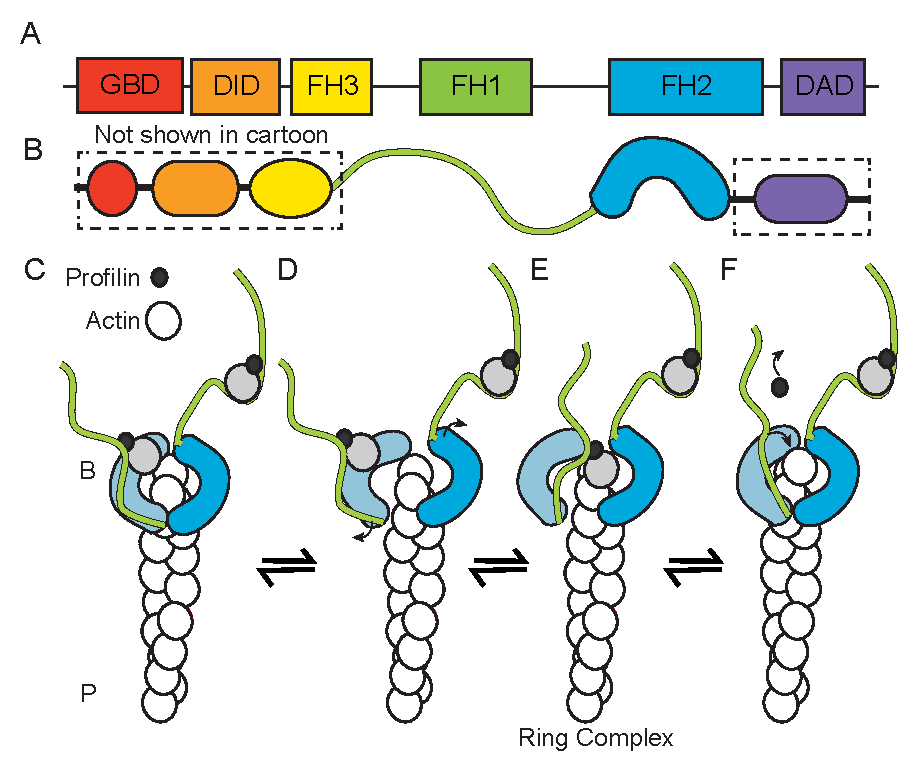
\includegraphics[width=13cm]{img/ch01/formin_mech.pdf}
\caption[Domain organization and stepping second mechanism of formins.]{\textbf{Domain organization and stepping second mechanism of formins.} (A-B) Domain organization and structure cartoon of formin. The N-terminal GTPase binding domain (GBD) binds to Rho-GTPase to release autoregulation by the Diaphanous inhibitory domain (DID) binding the Diaphanous autoregulatory domain (DAD). Formin Homology 1 (FH1) binds profilin-actin and can transfer it to the barbed end which is bound by a dimerized formin homology 2 (FH2) domain. Some formins also contain a formin homology 3 (FH3) domain involved in targeting. (C-F) Profilin-actin binds the FH1 domain and can be added to the barbed end of the filament (D) when the formin FH2 domains are in the open state. (E) A ring complex forms when the profilin actin is transferred from the FH1 domain to the FH2 barbed end. (E) Once the actin monomer is added to the filament, profilin dissociates, and then the FH2 domain translocates one step along the F-actin towards the barbed end.} 
\label{fig:formin-domain}
\end{figure}

\subsubsection{Ena/VASP}
Ena/VASP contains an N-terminal Ena-VASP homology 1 (EVH1) domain (Figure \ref{fig:ena-domain}A). This domain is important for localization within cells and binds to FP4 (FPPPP) motifs within such proteins as formin, zyxin, lamellipodin, vinculin \citep{ball_dual_2000, niebuhr_novel_1997, klostermann_orthologous_2000}. The EVH1 domain is present in all Ena/VASP family members as well as distantly related Wiskott-Aldrich syndrome proteins, WASP and N-WASP, and Homer/Vesl family, though proteins from outside the Ena/VASP family recognize different motifs. Structurally the EVH1 domain is similar to pleckstrin homology (PH) and phosphotyrosine-binding (PTB) domains, though there is little sequence similarity to these domains \citep{prehoda_structure_1999,reinhard_actin-based_2001,ball_dual_2000,fedorov_structure_1999}.
The C-terminal Ena/VASP Homology 2 (EVH2) domain contains the main actin interacting domains. The G-actin binding domain (GAB) is related to WH2 domains, which also bind actin monomers. The F-actin binding domain (FAB) is able to bind actin filaments while the C-terminal coiled-coil facilitates tetramerization. Between the EVH1 and EVH2 domain is a poly-proline region (PPR). This region can bind to profilin and other SH3 containing molecules such as Abl, Src \citep{lanier_abl_2000, gertler_mena_1996}. It is thought that profilin-actin can bind to both the GAB domain as well as the PPR to facilitate monomer addition to the barbed end \citep{ferron_structural_2007}. However, Ena/VASP is able to enhance elongation of F-actin without profilin present, in contrast to formins \citep{hansen_vasp_2010,breitsprecher_molecular_2011,winkelman_ena/vasp_2014,bruhmann_distinct_2017}.

\begin{figure}
\centering
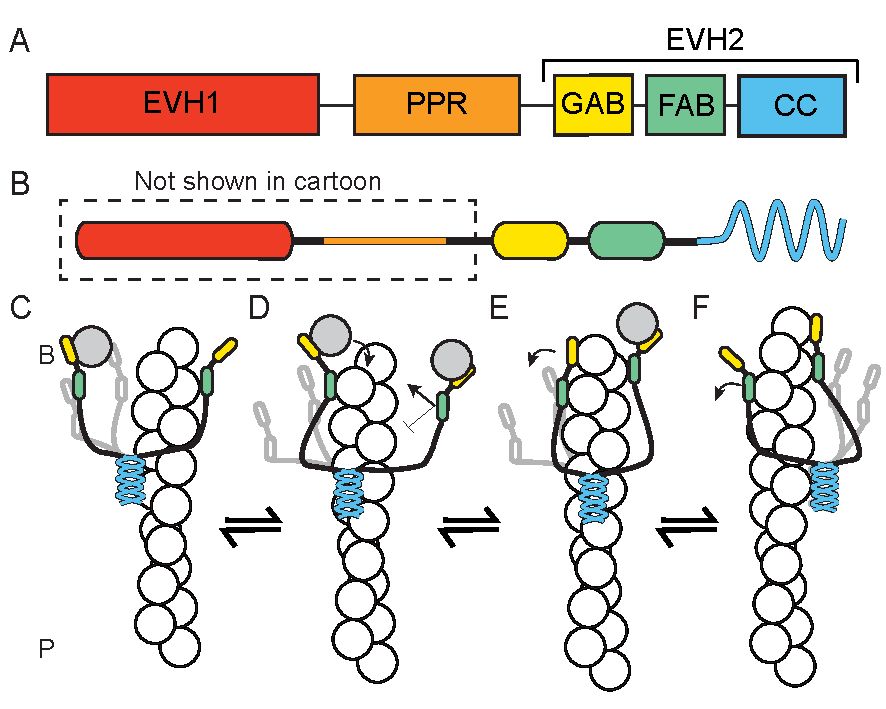
\includegraphics[width=13cm]{img/ch01/Ena_mech.pdf}
\caption[Domain organization and mechanism of Ena/VASP.]{\textbf{Domain organization and mechanism of Ena/VASP.} (A-B) Ena/VASP domain organization and cartoon structure of Ena/VASP: Ena/VASP homology domain 1 (EVH1, red), polyproline region (PPR, orange), Ena/VASP homology domain 2 (EVH2) includes G-actin binding domain (GAB, yellow), F-actin binding domain (FAB, green), coiled coil region (CC, blue). (C-F) Potential mechanism of Ena/VASP. (C) First G-actin binds the GAB domain that (D) can be transfered to the barbed end. Though only one monomer may be added at a time. (E) Once a monomer is added the GAB domain dissociates. (F) An 'arm' of Ena can bind to the side of the filament to prevent diffusion away from the barbed end while another monomer is added.}
\label{fig:ena-domain}
\end{figure}

\subsection{Mechanism of processive F-actin elongation}\label{ena-formin mechanism}

\subsubsection{Formin}

The observation that elongation of F-actin decreases in the presence of formins when no profilin-actin is present suggests that the FH2 domain 'gates' the addition of new actin monomers \citep{kovar_control_2006,otomo_structural_2005,vavylonis_model_2006}. This gating occurs through the FH2 being in a dynamic equilibrium between a tightly bound “closed” state and loosely bound “open” state. When the FH2 domain is in the closed state there is an over-rotation of the actin filament from the native F-actin state of $167^{\circ}$ to $180^{\circ}$. New actin monomers cannot be added while the FH2 domain is in the closed state due to this over-rotation because it does not contain favorable contacts for an incoming subunit at the barbed end \citep{otomo_structural_2005}.

There are two main models proposed for the formin processive elongation mechanism, stair-stepping and stepping second. Stair stepping, the first proposed model, begins with the FH2 in the closed state bound tightly to three actin subunits with four actin binding contacts. To transition to the open state the FH2 domain must dissociate two actin binding contacts and 'step' towards the barbed end. While in the open state, a monomer can bind to the F-actin barbed end and the FH2 domain at one of the recently dissociated binding sites. With the addition of a new monomer, the FH2 domain returns back to the closed state. Therefore, the stair stepping mechanism predicts that the FH2 domain translocates first, followed by monomer addition \citep{otomo_structural_2005}. Importantly, the translocation state is the most loosely bound state where formin would dissociate. In the stepping second model, monomer addition occurs first, then translocation of the FH2 domain can occur. The FH2 domain again starts in the closed state with four actin-binding contacts. Within an equilibrium, the FH2 domain releases two contacts with the barbed end to be in the open state which allows monomer addition, but cannot step in this open state. After a monomer binds to the barbed end, the formin is transiently bound to two interior subunits. The FH2 domain can then move onto the new barbed end by passing through a dissociative translocating state to return to the closed state binding the newly added monomer\citep{paul_role_2008,paul_review_2009} (Figure \ref{fig:formin-domain}B). The stair stepping model proposes that formin enters its most unstably bound (open) state independent of monomer addition, while the stepping second model predicts that formin only enters the dissociative state after monomer addition. Therefore the stepping second model predicts that formin's dissociation rate should be proportional to the number of actin monomers added whereas the stair stepping model predicts that dissociation should be a function of time \citep{paul_review_2009}. It was observed that formin dissociated as a function of the number of actin monomers added, lending support to the stepping second model \citep{paul_role_2008}. 

Whether the FH2 domain is in a closed or open state can dictate whether additional monomers can be added to the barbed end of a filament. Modulating the open-closed equilibrium state would allow fine-tuning of formin-mediated elongation rates. Using microfluidics, recent studies have shown that formin-mediated elongation rate is sensitive to tension on the formin and filament \citep{courtemanche_tension_2013,jegou_formin_2013}. Jégou et al. showed that the formin mDia1's elongation rate is increased up to two-fold when under tension. Similarly, Courtemanche et al. have shown that the elongation rate of the formin Bni1 also increases when a pulling force is applied, though only in the presence of profilin. Both groups suggest that a pulling force shifts the gating equilibrium of the FH2 domain towards the open state, which then causes an increase in elongation. Interestingly, when the FH1 domains are also pulled straight the elongation rate still increases. Therefore, the space that the FH1 can explore to find monomers is not a major factor because when the FH1 have reduced mobility you do not see reduced elongation rates.  The sensitivity to tension opens up the possibility that within cells formins can sense mechanotransduction of forces, which could tune formin elongation rates. A recent study by Zimmermann et al. showed formin mechanosensitivity, potentially localized in the FH1 domain in Cdc12. When myosin is used to pull on filaments being elongated by Cdc12, it causes Cdc12 to pause the filament's elongation. Even more surprising, mDia2 does not have this mechanosensitive property with elongation, suggesting this could be important for Cdc12's role in cytokinesis in fission yeast \citep{zimmermann_mechanoregulated_2017}. 

These models also predict that rotation must occur for formins to track the helical twist of the actin filament as it processively elongates filaments. However, early work suggested that this rotational tracking didn't occur, because formins stuck on a glass coverslip buckled rather than supercoil the actin that was adhered to the glass at its pointed end. To relieve the torque, it was proposed that the formin would 'slip' on the end of the F-actin \citep{kovar_insertional_2004,shemesh_novel_2005}. Recently, advances in microscopy have allowed us to gain a clearer understanding of formin rotation during elongation. Mizuno et al. found that helical rotation is an intrinsic property of formins intrinsically using fluorescence polarization. The observed a periodic oscillation of a sparsely tetramethylrhodamine (TMR) labeled filament elongated by a formin (mDia1) biotinylated to a surface. The periodic movement of the actin label corresponded to the long-pitch helical length of F-actin, therefore the actin filament was rotating. In this experimental setup, the the filament was forced to rotate rather than the formin because the formin was linked to the surface. However, \textit{in vivo} it is more likely that formins rotate rather than filaments during elongation, especially within crosslinked F-actin networks \citep{mizuno_rotational_2011}. This work raises many new questions including whether formin binding partners would rotate with the formins and if this would affect their actin assembly properties. It also opens new possibilities for mechanisms of regulation involving formin rotation. 

\subsubsection{Ena/VASP}
Ena/VASP can increase the elongation of F-actin using both actin monomers and profilin-actin \citep{kang_profilin_1997,hansen_vasp_2010, winkelman_ena/vasp_2014}. It is thought that profilin-actin loads on the PPR and GAB domain where actin monomers bind to the GAB domain. Profilin-actin has a higher affinity for the PPR than profilin alone which reduces non-efficient loading of profilin over profilin-actin \citep{ferron_structural_2007}. Furthermore, it was shown that profilin-actin has a higher affinity for the GAB domain than actin monomers alone, suggesting that Ena/VASP would elongate actin filaments using profilin-actin over free actin monomers \citep{chereau_understanding_2006}. However, even though profilin-actin is preferred, Ena/VASP can effectively elongate F-actin with only actin present \textit{in vitro} in contrast to formins \citep{hansen_vasp_2010,winkelman_ena/vasp_2014}. After being bound to an 'arm' of Ena via the PPR and GAB domains, the actin monomer or profilin-actin can then be added to the barbed end of the actin filament \citep{chereau_understanding_2006, ferron_structural_2007, breitsprecher_molecular_2011}. Once the actin monomer adds to the filament and undergoes a conformational change, the affinity of the GAB domain for the newly added monomer is reduced and is therefore released. Hansen et al. showed using VASP that the number of subunits added to the filament is proportional to the concentration of actin, while the dwell time is constant \citep{hansen_vasp_2010}. This is in contrast to formins that can only take a certain number of steps or equivalently add a certain number of monomers on average before dissociating. This presents an interesting extrapolation \textit{in vivo} where actin concentrations are higher and suggests that VASP could be more effective in the presence of these higher concentrations.  

Ena/VASP was originally thought to be processive clustered on beads \citep{breitsprecher_clustering_2008}, but was later observed to elongate actin filaments as single molecules in solution \citep{hansen_vasp_2010,winkelman_ena/vasp_2014, breitsprecher_molecular_2011}. It is not well understood how Ena/VASP is functioning in cells during filopodia initiation and maintenance. Ena/VASP is seen to localize in a cluster at the tips of filopodia, so the current model is that Ena/VASP is clustering at the plasma membrane in cells \citep{svitkina_mechanism_2003,lanier_mena_1999}. One open question about Ena/VASP's mechanism is whether it tracks the helical pitch of F-actin as it elongates, similar to the formin mDia1. Since Ena/VASP is thought to work in clusters and on bundled filaments in filopodia, our hypothesis is that instead of rotating along F-actin's helical pitch, Ena/VASP rather tip-tracks the barbed end of the filament. Furthermore, since Ena/VASP is a tetramer, understanding if all arms function in equal roles during filament elongation is also another open mechanistic question about Ena/VASP. 

\subsection{Behaviors}\label{ena-formin-behaviors}

\subsubsection{Formin}
The main functions of formins include F-actin nucleation, processive elongation, and actin filament crosslinking \citep{pollard_actin_2016}. However, there are multiple different formins in cells that are tuned for diverse processes. Each formin has a balance of the main functions as well as some additional properties that allows it to carry out the unique process. For example, there are three formin isoforms in fission yeast (Cdc12, Fus1, and For3) that are responsible for diverse actin networks. Each of these formins varied nucleation rates, processivity, elongation and ability to bundle. Cdc12 and Fus1 can efficiently nucleate filaments and are 70-fold better nucleators than For3 \citep{scott_functionally_2011}. Cdc12 and For3 are both highly processive and elongate filaments at a moderate rate, while Fus1 is only able to elongate filaments at half of this rate in the absence of profilin. Where Cdc12 adds 27 times more monomers than Fus1 on an average processive run, Fus1 is the only fission yeast formin that can bundle filaments. These varying behaviors of the different formin isoforms found within the same organism raises the question of how these formins are tuned to their unique role within the cell. Furthermore, how do proteins differentially interact with these formins, and how can that contribute to or change these properties?

The actin assembly activity of formins can also be tuned to the environment in the cell. Higashida et al. have shown that mDia1 rapidly increases processive F-actin assembly with the release of cell tension using sequential fluorescence decay after photoactivation (s-FDAPplus) to visualize the nucleation and elongation activity of mDia1 \citep{higashida_f-_2013}. A recent study from Zimmermann et al. showed that fission yeast Cdc12 is mechanoregulated by myosin. Cdc12-mediated elongation of F-actin is inhibited while the filament is under tension \citep{zimmermann_mechanoregulated_2017}. This plays an important role for fission yeast cytokinesis and was predicted by mathematical modeling of the process \citep{vavylonis_model_2006}. How actin and binding proteins are able to sense cell stress and forces is not very well understood. It will be important to look into what protein(s) are initially sensing the forces on the cell and how this is translated to modifying actin networks. 

Previous formin research has often focused on the two characteristic FH1 and FH2 domains to understand their actin assembly properties. However, formins contain other domains that vary across the formin family, including those that function in auto-regulation, inhibition, depolymerization, and filament actin (F-actin) binding. New studies have shown that the C-terminal tails of different formins play an important role in its actin assembly and nucleation properties. Cappuccino (Capu) \citep{vizcarra_role_2014}, FMNL3 \citep{heimsath_c_2012}, and mDia1 \citep{gould_formin_2011} can bind G-actin monomers with their C-terminal tails to help the FH2 domains nucleate F-actin filaments. Furthermore, Vizcarra et al. suggest that Capu's C-terminal tail also enhances elongation by forming nonspecific electrostatic interactions with F-actin that can assist in stabilizing the open-state FH2 dimer binding to the actin filament. INF2 has been shown to have important domains present in the C-terminal tail that can bind and sequester actin monomers \citep{chhabra_inf2_2006}. However, even though many formins depend on their C-terminal tail for their specific function, they do not all function equally. Replacing the C-terminal tail of Capu with the C-terminal tail of DRF formins changed its nucleation and processivity properties \citep{vizcarra_role_2014}. The growing evidences of the role of the C-terminal tail in tuning of nucleation and processivity opens up the possibility of differential regulation and function of formin isoforms present in the same cell. Whether these C-terminal interactions have important contributions to formin function and regulation overriding that of the FH1FH2 is unclear. 

Beyond binding to actin, Capu's C-terminal tail along with specific residues of the FH2 have been shown to promote high affinity microtubule binding, though this occurs separately from Capu's actin assembly properties \citep{roth-johnson_interaction_2014}. Actin and microtubule dynamics are linked within the cell and the details of this relationship remain a current question in the field. Recently it has been shown that formins mDia1, mDia2, and mDia3 are involved in ErbB2-dependent microtubule capture through their FH2 domains \citep{daou_essential_2014}. Additionally, TIRFM was used to visualize the interaction between microtubule plus end localizing CLIP-170 and formin mDia1, which stimulates actin growth from microtubule plus ends \citep{henty-ridilla_accelerated_2016}. This opens up many new questions about how various formins could be regulating actin-microtubule crosstalk. 

\subsubsection{Ena/VASP}
Ena/VASP's main function is an actin elongation factor. Studies of different Ena/VASP homologs have observed differences in the rate of actin elongation and time that Ena/VASP is bound to the barbed end \citep{breitsprecher_clustering_2008,breitsprecher_molecular_2011,hansen_vasp_2010,winkelman_ena/vasp_2014}. These properties are thought to be a tuning of the affinity of the GAB domain for actin, though differences in the FAB affinity could also play a role. Interestingly, mammalian paralogues can form heterotetramers through conservation of the coiled-coil domain \citep{riquelme_selectivity_2015}. However, this it was observed that the paralogues did not equally associate \textit{in vivo}. This opens up interesting questions about how different paralogues are regulated and how mixed heterotetramers effect processes in cells. 

While Ena/VASP is associated with barbed ends, it can compete with capping protein. However, once capping protein binds to the barbed end Ena/VASP cannot uncap the filament \citep{applewhite_ena/vasp_2007, bear_ena/vasp:_2009, winkelman_ena/vasp_2014,barzik_ena/vasp_2005}. This function is thought to be important in cells as Ena/VASP is localized to the leading edge of motile cells as well capping protein. Especially within the convergent elongation model for filopodia formation, this competition for capping protein allows some of the short filaments within the lamellipodium to be protected and elongated, facilitating filopodia initiation \citep{svitkina_mechanism_2003}. 
In addition to barbed end binding, Ena/VASP has been shown to bundle filaments, especially at higher concentrations \textit{in vitro} \citep{bachmann_evh2_1999,barzik_ena/vasp_2005}. However, it is not known how important this function is in cells since Ena/VASP is seen to localize to filopodia tips and not the shaft as fascin does \citep{svitkina_mechanism_2003,lanier_mena_1999}. Another function of Ena/VASP observed \textit{in vitro} is nucleation. Ena/VASP has been shown to nucleate filaments in bulk assays, yet \textit{in vivo} experiments have not shown that this is a physiological function \citep{bear_ena/vasp:_2009}. Both of these functions have been shown to be salt dependent, so one possibility is that at physiological conditions these activities are very weak. 

\subsection{Regulation}\label{ena-formin-regulation}

\subsubsection{Formin}
It is well established that DRF formins are autoregulated by interaction of the DID-DAD domains, which can be relieved by Rho-GTPase binding. Recently, a structure has been solved of full-length mDia1 that confirms that the DID-CC domain sterically occludes where actin binds on FH2 during nucleation \citep{maiti_structure_2012}. Furthermore, it was shown that the formin does not quickly return to its autoinhibited state during processive elongation, which opens further questions about how, or if, formins are stopped once a processive run has been initiated. Other insights into autoregulation have been highlighted by the structure of Rho-GTPase Cdc42 with formins FMNL1 and FMNL2. The structure along with biochemical data suggests that specific interactions between formin FMNL2 and the Rho-GTPase insert helix are at play when determining specificity of Rho-GTPases to release formin autoinhibition \citep{kuhn_structure_2015}. Beyond autoregulation, it has been shown that PIP2 can inhibit mDia1 by binding to its C-terminal tail. Phospholipids can recruit mDia1 to the membrane \citep{van_gisbergen_class_2012}, which then causes an accumulation of PIP2 so phospholipids are able to regulate formin localization to the membrane and inactivation \citep{ramalingam_phospholipids_2010}. 

Recent studies focusing on formin binding partners has opened up even further opportunities for regulation. The formin mDia1 can interact with adenomatous polyposis coli (APC) through its tail, forming a complex that acts as a potent nucleator \citep{breitsprecher_rocket_2012,okada_adenomatous_2010}. Likewise, nucleation-promoting factor Bud6 is known to enhance the nucleation of formin Bni1 \citep{moseley_differential_2005}. Capu and closely related FMN2 have been shown to interact with the nucleating protein Spire with their C-terminal domains \citep{montaville_role_2016,montaville_spire_2014, pechlivanis_identification_2009,vizcarra_structure_2011}. Recent studies have visualized a 'decision complex' of capping protein and formins mDia1 and FMNL2. Previous genetic and biochemical work suggested that formins and capping protein were entirely antagonistic \citep{kovar_profilin-mediated_2005}, yet single-molecule TIRF microscopy has shown that both of these proteins can bind simultaneously to a barbed end for a set amount of time before one gains sole control \citep{bombardier_single-molecule_2015,shekhar_formin_2015}. Further questions remain about how different formins are regulated to act at the precise time and location within a cell. Exploring the interaction between a formin and different protein binding partners and macromolecules can open up new possibilities for regulation.

\subsubsection{Ena/VASP}
Ena/VASP proteins were originally identified as substrates for different kinases \citep{halbrugge_analysis_1990,gertler_genetic_1990}. Additional studies have shown that vertebrate Ena/VASP are substrates for cAMP- and cGMP-induced protein kinases with serine/threonine phosphorylation sites in both the PPR and EVH1 domain, with the latter being the preferred site \citep{gertler_mena_1996,lambrechts_camp-dependent_2000,harbeck_phosphorylation_2000,butt_camp-_1994}. Phosphorylation at these sites have shown decreased Ena/VASP activity both \textit{in vitro} and \textit{in vivo} \citep{loureiro_critical_2002,howe_regulation_2002,benz_differential_2009,butt_camp-_1994}. 
Beyond regulation by phosphorylation, different isoforms of profilin can affect the activity of Ena/VASP \citep{hansen_vasp_2010,mouneimne_differential_2012}. Different mammalian Ena/VASP proteins are able to utilize specific isoforms of profilin to increase their activity. This specificity, along with the ability of mammalian paralogues to form mixed tetramers, could result in a tunable system based on the Ena/VASP monomers and profilin isoform spatial-temporal localization in cells. 

\subsection{Ena/VASP and formin interaction}\label{ena-formin-interaction}
Although their biochemical mechanisms and rate constants are quite different, Ena/VASP and formins both stimulate the assembly of long, straight filaments within cells in two ways: both families 1) protect actin filaments from capping protein by processive association with the barbed end and 2) increase elongation rate of filaments during this processive association. In line with these activities, both protein families induce the assembly of filopodia \citep{bilancia_enabled_2014,homem_exploring_2009} and localize to zones of actin assembly at distal tips of these structures. However, Ena/VASPs and formins appear to drive distinct types of filopodia \citep{barzik_ena/vasp_2014,bilancia_enabled_2014,nowotarski_actin_2014,homem_exploring_2009}. In general, formin-induced filopodia are much longer, and the actin is not highly connected with other actin networks. Conversely, Ena/VASP-induced filopodia are shorter and deeply rooted in lamellar networks. During dorsal closure in fly embryos, motile epithelial cells displayed filopodia more characteristic of Ena, while underlying non-motile amnioserosal cells displayed filopodia more characteristic of formin Dia \citep{nowotarski_actin_2014}. However, both proteins played roles in both tissue types. It is possible that in each tissue type, activities of each elongation factor are modulated accordingly to drive different functions. For example, it has been suggested that Ena/VASP may work primarily in reorganizing preexisting networks in the leading edge of motile cells through a convergent elongation-type mechanism \citep{svitkina_mechanism_2003}. Formin, which can also nucleate actin filaments, may not require a preexisting lamellipodial network and assemble its own filaments for filopodia de novo \citep{faix_filopodia:_2009}, and therefore may function more in non-motile cells. 

However, Ena/VASPs and formins directly bind to each other and colocalize at the distal tips of some filopodia. These observations led different groups to question why these proteins with generally similar assembly properties would colocalize in filopodia and how their direct binding might regulate each other's activity. Ena/VASP's EVH1 domain mediates this interaction either through formin's FH1 \citep{bilancia_enabled_2014} and/or FH2 domain \citep{barzik_ena/vasp_2014,schirenbeck_bundling_2006}. Ena's EVH1 domain binds to the fly formin Diaphanous with a Kd of 13 $\mu$M, similar to the low affinity EVH1-FPPP4 interaction that the EVH1 uses to bind a large number of other proteins \citep{prehoda_structure_1999}. This interaction may negatively regulate formin by interfering with the core assembly machinery. 

Recent data shows that in addition to Ena/VASP and formin driving distinct filopodial morphology and dynamics, Ena/VASP is necessary for proper function in some cells. Bilancia et al., found that Ena could negatively regulate the formin Diaphanous both in vivo and in vitro \citep{bilancia_enabled_2014}. Work from the Gertler lab extended these ideas by showing the physiological consequences of driving filopodia formation with either formin or Ena/VASP \citep{barzik_ena/vasp_2005}. This study found that although formins can generate filopodia, Ena/VASP is necessary for initiating focal contacts and integrin-dependent signaling. It is not currently clear if these dynamics play out in all cell types, and will be an important area of future research. In addition, the effect of formin on Ena/VASP activity, if any, is also an area of future research.

\section{Single-molecule total internal reflection microscopy (TIRFM)}\label{tirfm}
The main experimental set-up that we have used to study actin binding proteins and their activity and dynamics is total internal reflection microscopy (TIRFM). This microscopy uses a special objective that allows for a low angle of incidence of the incoming laser. The laser internally reflects between the glass slide and coverslip. This internal reflection causes an evanescent wave that can illuminate fluorophores within 150 $\mu$m from the coverslip. By only illuminating this small area, we get much better signal to noise by reduction of background fluorescence beyond the 150 $\mu$. TIRFM is especially beneficial for observing single molecules due to the reduced background. Single-molecule TIRFM allows us to measure single events at low concentrations of our protein of interest \citep{zimmermann_vitro_2016,fish_total_2009}. Specifically for studying the actin cytoskeleton, we are able to watch filaments assemble in real time and monitor binding dynamics and how actin binding proteins interact with F-actin. Compared to bulk actin assays such as fluorescent pyrene assays we are able to distinguish polymerization, nucleation, and measure actual elongation rates of the filaments. We are also able to localize where proteins are interacting with the actin filament as well as other actin binding proteins. One of the biggest advantages of visualizing actin binding proteins with TIRFM is the ability to measure dynamics of both binding and dissociation of the F-actin. This kinetic information can inform the molecular mechanisms of actin binding proteins.

\begin{figure}
\centering
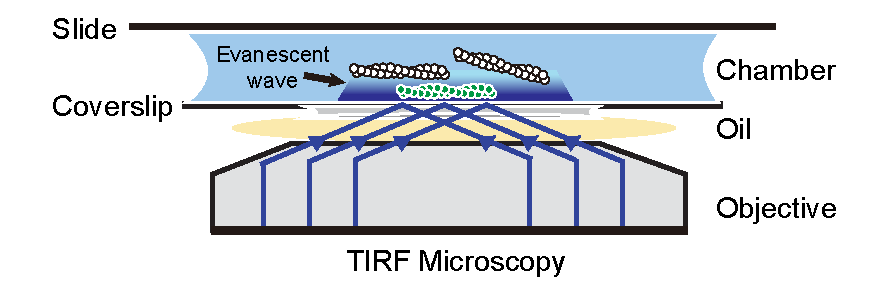
\includegraphics[width=17cm]{img/ch01/tirf_thesis.pdf}
\caption[Diagram of Total Internal Reflection Fluorescence Microscopy (TIRFM)]{\textbf{Diagram of Total Internal Reflection Fluorescence Microscopy (TIRFM)} Total Internal Reflection Fluroesence Microscopy (TIRFM) consists of a fluorescent sample being placed in a flow chamber between a coverslip and glass slide. The flow chamber is placed on an oil objective and visualized using a laser at a critical angle that allows for total reflection within the coverslip, forming an evanescent wave that only excited fluorophores within a few hundred nanometers of the coverslip. }
\label{fig:tirf}
\end{figure}